\chapter{Synthetic ultraviolet flux maps of M31 from resolved optical
    photometry.
}
\label{m31flux}

\begin{quote}
\begin{center}
\textbf{\large Abstract}
\end{center}

We have used color-magnitude diagram-based star formation histories (SFHs) and
stellar population synthesis to create maps of synthetic ultraviolet (UV) flux at
sub-kpc resolution for the northeast quadrant of M31. We then compared the
synthetic flux maps with observations from GALEX.

\end{quote}


\section{Introduction}

M31 is well-studied and has been observed at a variety of wavelengths, e.g., in
the ultraviolet (UV) by the Galaxy Evolution Explorer
\citep[GALEX][]{Morrissey:2007}, in the optical, including H$\alpha$, for the
Local Group Galaxies Survey \citep{Massey:2006}, and in the infrared by the
Spitzer Space Telescope \citep{Gordon:2006}. The wealth of high-quality data
available for M31 provides a valuable opportunity to model the observations and
test our current understanding of stellar astrophysics. In particular, the
initial mass function (IMF), stellar evolution and spectra models, and
extinction curves are all required to model the light produced by a galaxy.

A critical ingredient for modeling the flux from a galaxy is a detailed
knowledge about its underlying star formation history (SFH). Deriving SFHs by
color-magnitude diagram (CMD) analysis is a reliable method that can be used
whenever photometry of resolved stars are available. An extensive optical
photometric catalog for M31 has been compiled by the Panchromatic Hubble
Andromeda Treasury \citep[PHAT][]{Dalcanton:2012}, and \citet{Lewis:2014} have
used these data to derive the spatially-resolved SFH of the northeast quadrant
of M31. With sub-kpc resolution, this SFH dataset is the ideal input for
stellar population synthesis codes that model total flux given a population's
star formation rate (SFR) and metallicity evolution. The result is a set of
spatially-resolved maps of synthetic broadband flux in M31 which can be
compared with observations.

The \citet{Lewis:2014} SFHs can also be used to create temporally-average SFR
maps. Because the SFHs were derived from the resolved stars without any prior
assumptions about the SFHs, such maps provide a standard against which
flux-based SFR estimates \citep[e.g., using any of the calibrations
from][]{Kennicutt:2012} can be tested. Using integrated flux to estimate SFRs
for distant galaxies where resolved stars are not available is a common
technique in extragalactic astronomy. Some studies have investigated how
flux-based SFR estimators hold up against resolved-star SFHs in sub-kpc
UV-bright regions \citep{Simones:2014} and in low-metallicity dwarf galaxies
\citep{McQuinn:2014}, yet relatively little attention has been paid to the
accuracy of such estimators in general.

In this study, we have used the PHAT CMD-based SFHs and stellar population
synthesis to create maps of synthetic ultraviolet (UV) flux at sub-kpc
resolution for the northeast quadrant of M31. We then compared the synthetic
flux maps with observations from GALEX. We currently only focus on GALEX \fuv{}
and \nuv{} (far and near UV), though this work can easily be extended to other
wavelength regimes. In \S \ref{mfx:syntheticfluxmaps}, we describe the SFH
dataset and the production of the synthetic flux maps. \S
\ref{mfx:observations} describes the process of producing observed flux maps
from GALEX \fuv{} and \nuv{} images. The creation of SFR maps both from the
SFHs and the observed fluxes using common flux-SFR calibrations are described
in \S \ref{mfx:sfrestimates}. In \S \ref{mfx:discussion}, we compare the
synthetic maps with the observations and compare mean SFR maps with SFRs
estimated from observed flux. We conclude in \S \ref{mfx:conclusion}.

\textbf{*** TODO}

\begin{enumerate}
\item What am I missing here? Make sure to mention previous work addressing our
    science questions. Leave this alone for now; our science questions won't be
    completely defined until the discussion is complete.
\end{enumerate}

\textbf{***}





\section{Synthetic UV flux maps}\label{mfx:syntheticfluxmaps}



\subsection{The spatially-resolved star formation history of M31}

\citet{Lewis:2014} used \acsb{} and \acsi{} Hubble Space Telescope
(HST)/Advanced Camera for Surveys (ACS) photometry of over 100 million stars
from the PHAT survey \citep{Dalcanton:2012} to derive spatially-resolved SFHs
for the northeast quadrant of M31, excluding the crowded bulge area. To
summarize their work, each brick (using PHAT terminology; see Figure
\ref{fig:mfx:dummy1}) in the PHAT survey (excepting bricks 1 and 3) was divided
into 450 regions on a uniform $15 \times 30$ grid, with each region $\sim
24\aarcsec \times 27\aarcsec$ in size. The $\acsb,\acsi$ CMD of each region was
then fit by MATCH \citep{Dolphin:2002} to determine the most likely SFH under
the following assumptions:

\begin{enumerate}
\item The \citet{Kroupa:2001} IMF.
\item The Padova isochrones \citep{Marigo:2008} with updated asymptotic giant
    branch tracks \citep{Girardi:2010}.
\item A binary fraction of 0.35 with a uniform secondary mass distribution.
\item A distance modulus of 24.47 \citep{McConnachie:2005}.
\item An age resolution of $0.1\dex$ over the range $6.60 \le
    \logten(\mathrm{age}) \le 9.90$.
\item A metallicity resolution of $0.1\dex$ over the range $-2.3 \le \met \le
    0.1$, constrained to increase over time.
\item A two-parameter extinction model with foreground (\avf{}) and
    differential (\dav{}) components, where the \avf{} and \dav{} parameters
    were optimized for each cell \citep[see also][]{Simones:2014}.
\end{enumerate}

In addition, the modeled CMDs were optimized to the main sequence by excluding
all stars with $\acsb - \acsi > 1.25$ and $\acsb > 21$ from the fit.


\begin{figure}
\centering

\includegraphics[scale=1.0]{m31flux-figures/dummy.pdf}
\caption[PHAT survey map.]{Map of the PHAT survey, showing the 21 bricks and
    maybe the region grid in one of the bricks.
}
\label{fig:mfx:dummy1}
\end{figure}



\subsection{Broadband UV flux modeling}\label{mfx:syntheticfluxmaps:fluxmod}

We used the SFH dataset from \citet{Lewis:2014} to model broadband fluxes in
various filters, allowing us to create synthetic flux maps for the PHAT survey
area. Past studies have used CMD-based SFHs to model fluxes, including
\citet{Gogarten:2009} for UV-bright regions in the outer disk of M81,
\citet{Johnson:2013} for dwarf galaxies in the Local Volume, and more recently
\citet{Simones:2014} for a small sample of UV-bright regions in M31. Our work
builds on the analysis of \citet{Simones:2014} by extending our coverage to the
entire PHAT survey area to include a wide variety of environments. We chose to
focus on modeling fluxes in the GALEX \fuv{} and \nuv{} filters only (see Table
\ref{tab:mfx:filters}), though because we begin by modeling spectral energy
distributions (SEDs), the process we describe below can easily be generalized
to derive fluxes in any set of filters.

The modeling of broadband flux for a given region in the $15 \times 30$ grid of
a given PHAT brick is based on the technique described in \citet{Johnson:2013}.
We began with a set of simple stellar population (SSP) models generated using
the Flexible Stellar Population Synthesis (FSPS) code \citep{Conroy:2009,
Conroy:2010}. For consistency with \citet{Lewis:2014}, we ran FSPS assuming the
\citet{Kroupa:2001} IMF and the Padova isochrones \citep{Marigo:2008} with
updated asymptotic giant branch tracks \citep{Girardi:2010}. We also chose the
were BaSeL 3.1 semi-empirical stellar SED library \citep{Westera:2002}. The
SSPs were aged from $\log(\mathrm{age})=5.500$ to 10.175 in steps of
$0.025\dex$. We set the SSP metallicities independently for each region
depending on its SFH as either the mean metallicity over the last $100\myr$ of
the SFH, or the most recent metallicity where $\sfr > 0$ if all SFRs over the
last $100\myr$ were zero (we chose the $100\myr$ timescale because it
corresponds to the lifetime of UV emission).

We applied the SSP models to a region's SFH to model its integrated SED. We
first processed the SFH into a suitable form by rescaling the first age bin to
include all ages up to the present, and increasing the age resolution of the
full SFH to 20 samples per age bin. The subsampled SFH was then interpolated to
the series of ages in the set of SSP models. The SED of each SSP was weighted
by its corresponding mass from the SFH, and the individual SSP SEDs were
finally summed to derive the integrated intrinsic (i.e., unreddened) model SED
for the region.

We derived a reddened SED for the region using the same two-component
extinction model used by MATCH to fit the CMD together with the region's
best-fit \avf{} and \dav{} parameters \citep{Lewis:2014}. To do this, we
divided the intrinsic SED into 30 identical component SEDs (larger numbers of
components did not significantly improve the accuracy of our results). Each
component was reddened according to the \citet{Cardelli:1989} extinction curve
with a uniform random $A_\mathrm{V}$ drawn between \avf{} and $\avf + \dav$.
The \citet{Cardelli:1989} extinction curve predicts the amount of extinction
relative that in the V band, $A_\mathrm{V}$, as a function of wavelength and is
based on the average extinction in the Galaxy with a total-to-selective
extinction ratio of $\rv = 3.1$. Finally, the reddened SED components were
summed back together to obtain the region's integrated reddened model SED.

The intrinsic and reddened model SEDs were convolved with the response curves
for the GALEX \fuv{} and \nuv{} filters to obtain absolute \fuv{} and \nuv{}
magnitudes. These were converted into apparent magnitudes for the region by
projecting to a distance modulus of 24.47 \citep{McConnachie:2005}, consistent
with \citet{Lewis:2014}. We used the apparent magnitudes and the appropriate
magnitude-to-flux conversion formulae (see Table \ref{tab:mfx:filters}) to
derive the intrinsic and reddened broadband UV fluxes for the region. We denote
the intrinsic \fuv{} and \nuv{} fluxes by \ffuvsfhz{} and \fnuvsfhz{}, and the
reddened \fuv{} and \nuv{} fluxes by \ffuvsfh{} and \fnuvsfh{}, respectively.


% Table 1
\begin{deluxetable}{cccc}
\tabletypesize{\footnotesize}
\tablecaption{Filter constants and image names.\label{tab:mfx:filters}}
\tablewidth{0pt}
\tablehead{
    \colhead{Filter} &
    \colhead{$(\erg\ssec^{-1}\cm^{-2}\ang^{-1})/(\mathrm{counts}\ssec^{-1})$} &
    \colhead{AB mag zeropoint} &
    \colhead{Images}
}
\startdata
GALEX FUV &  $2.40 \times 10^{-15}\,\tablenotemark{a}$ &  18.82\tablenotemark{a} &  PS\_M31\_MOS00-fd-int.fits \\
          &                                            &                         &  PS\_M31\_MOS07-fd-int.fits \\
          &                                            &                         &  PS\_M31\_MOS08-fd-int.fits \\
          &                                            &                         &  PS\_M31\_MOS10-fd-int.fits \\
GALEX NUV &  $2.06 \times 10^{-16}\,\tablenotemark{a}$ &  20.08\tablenotemark{a} &  PS\_M31\_MOS00-nd-int.fits \\
          &                                            &                         &  PS\_M31\_MOS07-nd-int.fits \\
          &                                            &                         &  PS\_M31\_MOS08-nd-int.fits \\
          &                                            &                         &  PS\_M31\_MOS10-nd-int.fits
\enddata
\tablenotetext{a}{http://galexgi.gsfc.nasa.gov/docs/galex/FAQ/counts\_background.html}
\end{deluxetable}



After modeling the intrinsic and reddened fluxes for all of the regions in a
brick, we assembled the flux values (for a given filter) into a $15 \times 30$
array to form an image mapping the synthetic flux across the brick. The brick
map was independently tied to a world coordinate system using a 2D
least-squares optimization to find the best-fit CD matrix
\citep{Calabretta:2002} for the known RA and dec coordinates of the brick grid
vertices \citep[measured by][]{Lewis:2014}, assuming a gnomonic tangent plane
projection. We repeated this process for all of the \citet{Lewis:2014} bricks,
resulting in a set of 21 brick maps. We then reprojected and added the brick
maps using Montage\footnote{http://montage.ipac.caltech.edu/} to create full
maps, or mosaics, of synthetic \fuv{} and \nuv{} flux for the PHAT survey area.

All of the mosaic maps are registered to a grid defined by a template header
that was automatically chosen by Montage as the best fit to the collection of
input brick maps. The mosaic grid has a pixel scale of $23.75\aarcsec$, which
is comparable to the size of the original brick grids defined in
\citet{Lewis:2014}. Assuming a distance modulus of 24.47
\citep{McConnachie:2005}, a disk inclination of $78\ddeg$ \citep{Tully:1994},
and a position angle of $35\deg$ \citep{deVaucouleurs:1995}, the pixel scale is
deprojected to a linear size of $dx = 440\pc$ and $dy = 100\pc$ approximately
along the minor and major axes of M31, respectively. The synthetic flux maps
therefore have a resolution that is firmly in the sub-kpc regime.

The final synthetic \fuv{} and \nuv{} flux maps are shown in Figures
\ref{fig:mfx:modfluxmaps_fuv} (\ffuvsfhz{} and \ffuvsfh{}) and
\ref{fig:mfx:modfluxmaps_nuv} (\fnuvsfhz{} and \fnuvsfh{}).

We used the synthetic flux maps to derive maps of \afuv{} and \anuv{}, the
total extinctions in the \fuv{} and \nuv{} bands, respectively. The intrinsic
and reddened flux maps were converted into AB magnitudes (Table
\ref{tab:mfx:filters}), \fuvsfhz{} and \fuvsfh{} for the \fuv{} filter, and
\nuvsfhz{} and \nuvsfh{} for the \nuv{} filter. The extinction maps were then
calculated as the difference between the intrinsic and reddened magnitudes,
$\afuv = \fuvsfh - \fuvsfhz$ and $\anuv = \nuvsfh - \nuvsfhz$. We show the
modeled extinction maps with their corresponding synthetic flux maps in Figures
\ref{fig:mfx:modfluxmaps_fuv} and \ref{fig:mfx:modfluxmaps_nuv}.

A pixel weights map representing the coverage of the available PHAT data was
also produced during the mosaicking process. Mosaic pixels fully within the
PHAT survey border (excluding bricks 1 and 2 near the bulge) have a weight of
1, pixels fully outside the border have a weight of 0, and all other pixels
have weights between 0 and 1 depending on the fraction of the pixel area within
the survey border. This weights map is used to more accurately match the
synthetic flux maps with observations.


\begin{figure}
\centering
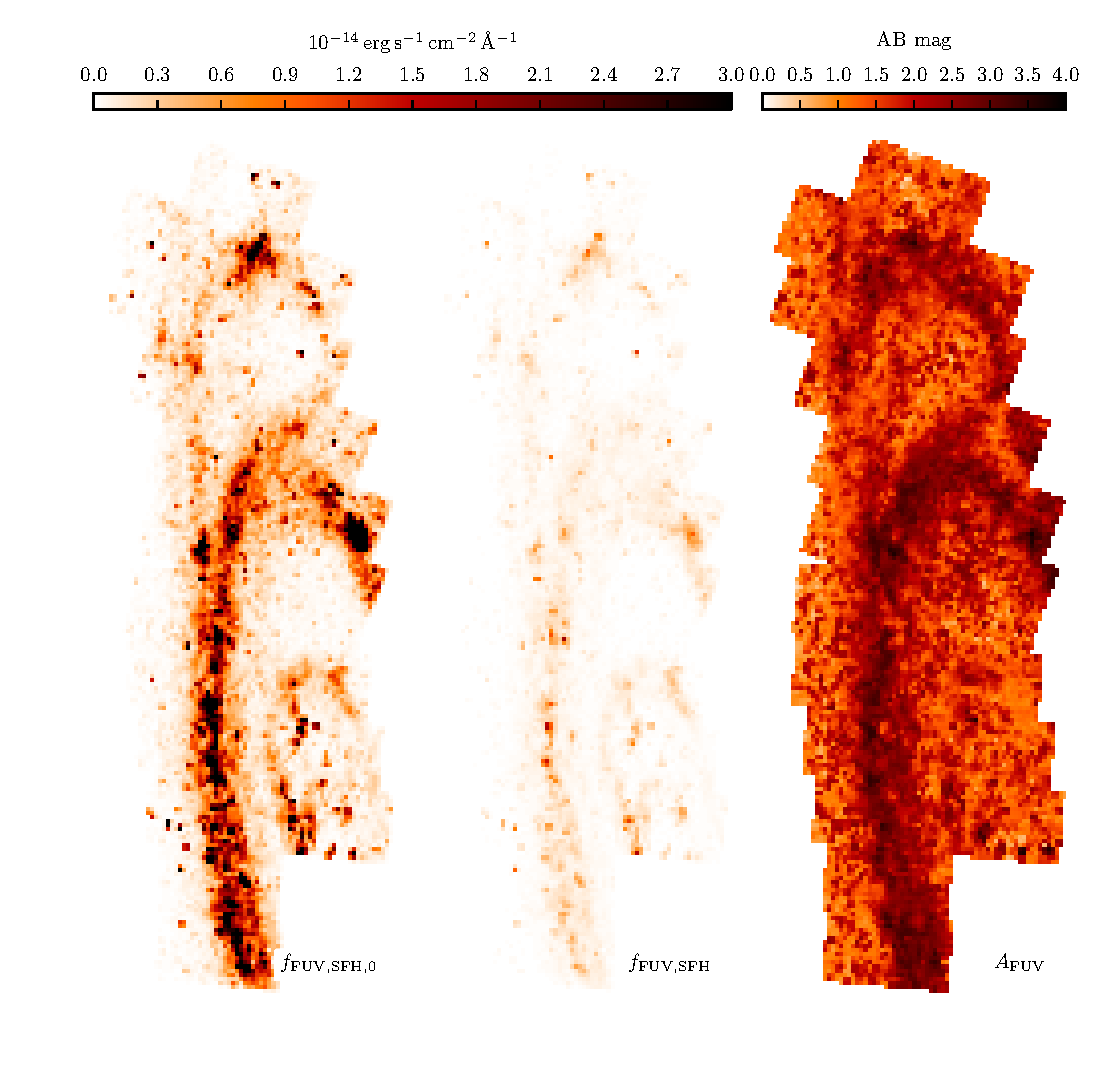
\includegraphics[width=\textwidth]{m31flux-figures/modfluxmaps_fuv.pdf}
\caption[\fuv{} flux map modeled from the SFHs.]{\fuv{} flux modeled from the SFHs.
    The intrinsic flux, \ffuvsfhz{}, is shown in the left panel and the middle
    panel shows the flux reddened according to the extinction model, \ffuvsfh{}
    (also shown alongside the observed GALEX \fuv{} flux in Figure
    \ref{fig:mfx:fluxmaps_fuv}). The \fuv{} extinction, \afuv{}, derived from
    \ffuvsfhz{} and \ffuvsfh{} is shown on the right.
}
\label{fig:mfx:modfluxmaps_fuv}
\end{figure}


\begin{figure}
\centering
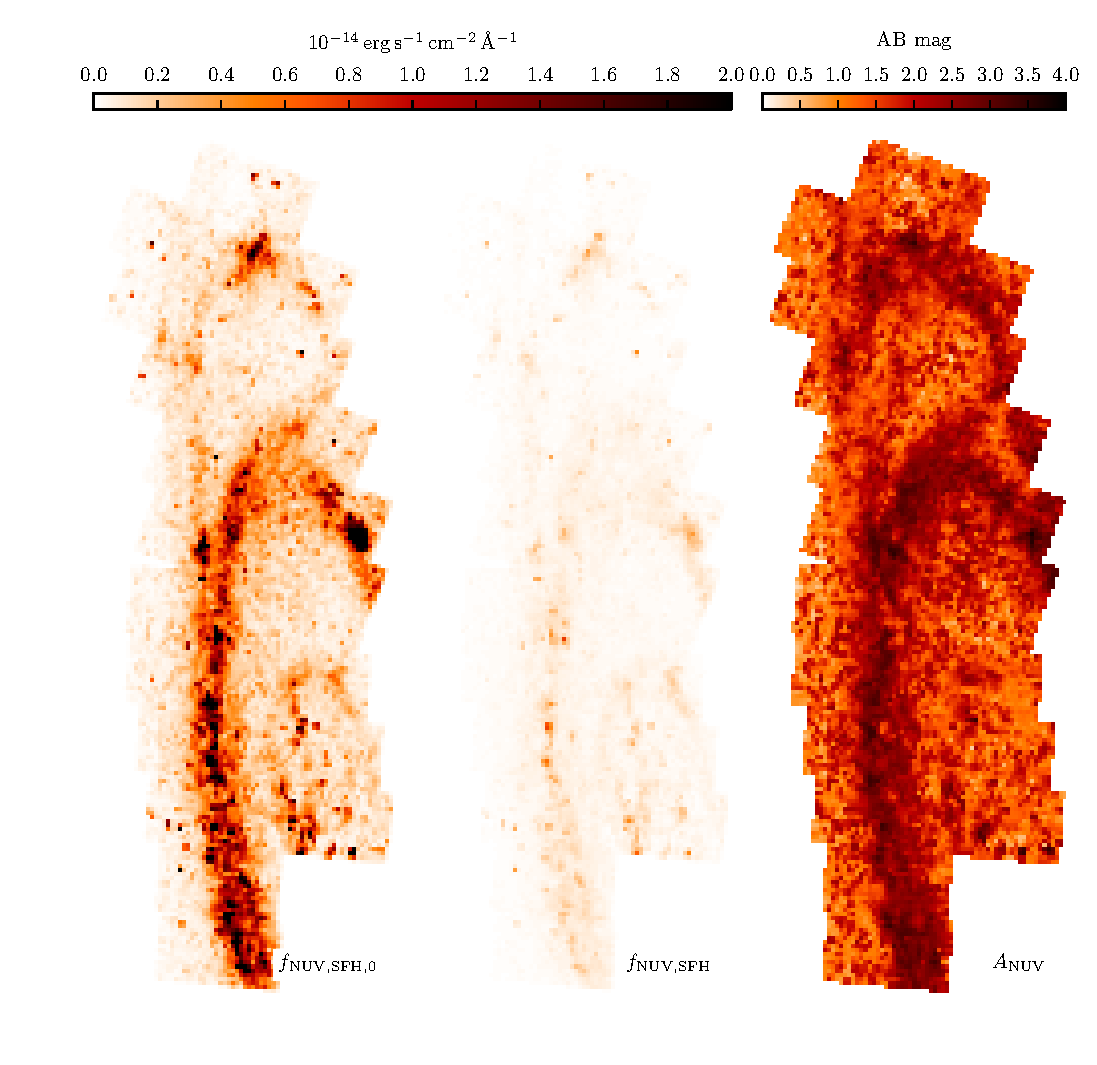
\includegraphics[width=\textwidth]{m31flux-figures/modfluxmaps_nuv.pdf}
\caption[\nuv{} flux map modeled from the SFHs.]{Same as Figure
    \ref{fig:mfx:modfluxmaps_fuv}, but for \nuv{} flux.
}
\label{fig:mfx:modfluxmaps_nuv}
\end{figure}

\textbf{*** TODO}

\begin{enumerate}
\item Uncertainties? The SFHs have statistical uncertainties from the CMD
    fitting process due to imperfect knowledge of the true underlying SFH that
    produced the observed CMD. There are also systematic uncertainties due to
    the optimization of \avf{} and \dav{}. Do we propagate these through to the
    modeled fluxes, or do we only care about the observational uncertainties
    (such as in Bayesian analyses where we evaluate the probability of the
    model given the data and its uncertainties)?
\item Make sure to add a footnote somewhere indicating that FITS files for the
    synthetic flux maps, and all of the other maps in this paper, are hosted on
    github.
\end{enumerate}

\textbf{***}





\section{Observations}\label{mfx:observations}

We constructed maps of observed GALEX \fuv{} and \nuv{} flux to match the
synthetic flux maps described in \S \ref{mfx:syntheticfluxmaps:fluxmod}. We
started with the intensity maps of four tiles in the GALEX Deep Imaging Survey
(DIS) covering the PHAT survey area (see Table \ref{tab:mfx:filters}). The
tiles were converted from units of $\mathrm{counts} \ssec^{-1}
\,\mathrm{pixel}^{-1}$ into flux using the factors in Table
\ref{tab:mfx:filters}. We then used Montage to reprojected the flux tiles to
the same template header as the synthetic flux mosaics (see \S
\ref{mfx:syntheticfluxmaps}). The individual tiles had slightly different
background levels, so we had Montage automatically match the backgrounds before
adding the tiles to form the final mosaic.

A small amount of background UV flux was present in the \fuv{} and \nuv{}
mosaics, primarily due to scattering of UV photons from hot stars in the
Galaxy. We measured the mean background flux in a rectangular aperture in an
off-galaxy area relatively devoid of stars in the reprojected, background
matched tile PS\_M31\_MOS07. The measured background values were $3.69 \times
10^{-19}$ and $5.88 \times
10^{-19}\erg\ssec^{-1}\cm^{-2}\ang^{-1}\aarcsec^{-2}$ ($2.5 \times 10^{-16}$
and $2.3 \times 10^{-16}\erg\ssec^{-1}\cm^{-2}\ang^{-1}$ per mosaic pixel) in
\fuv{} and \nuv{}, respectively. We subtracted these values from the \fuv{} and
\nuv{} mosaics to obtain the final observed UV flux maps for the PHAT survey
area. The observed \fuv{} flux, \ffuvobs{}, is shown in Figure
\ref{fig:mfx:fluxmaps_fuv} and the observed \nuv{} flux, \fnuvobs{}, is shown
in Figure \ref{fig:mfx:fluxmaps_nuv}.


\begin{figure}
\centering
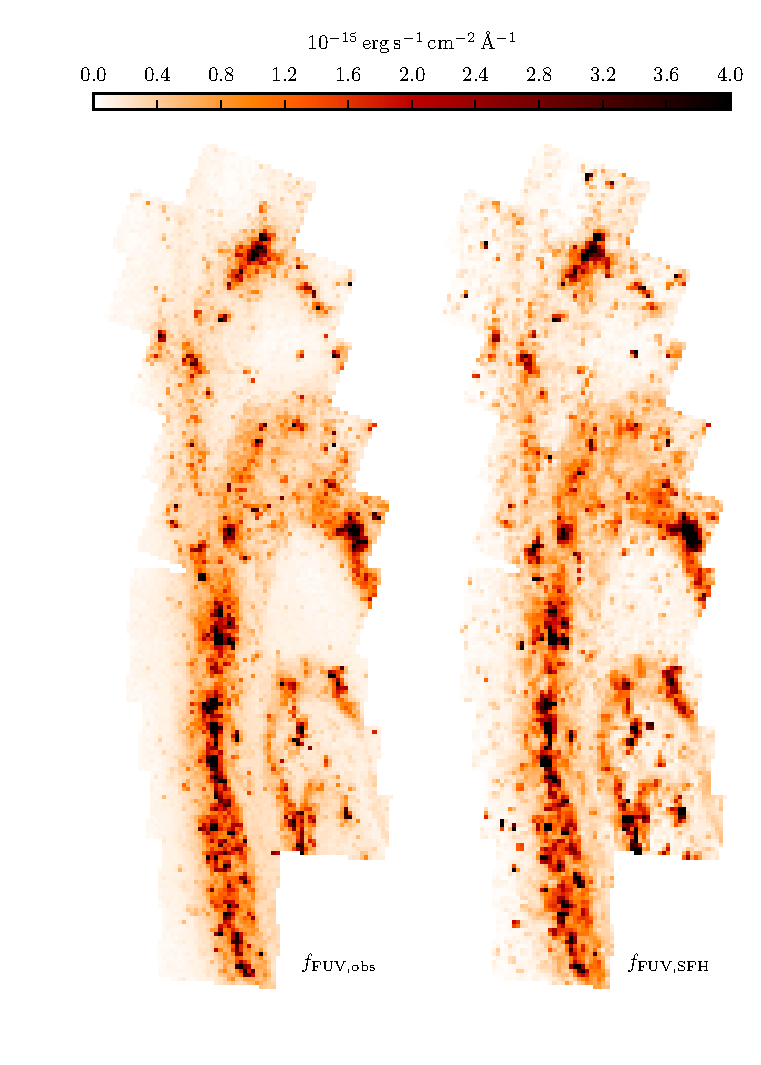
\includegraphics[width=\textwidth]{m31flux-figures/fluxmaps_fuv.pdf}
\caption[Observed and synthetic reddened \fuv{} flux maps.]{Observed \fuv{} flux from
    GALEX, \ffuvobs{} (left), and synthetic reddened \fuv{} flux from the SFHs,
    \ffuvsfh{} (right).
}
\label{fig:mfx:fluxmaps_fuv}
\end{figure}


\begin{figure}
\centering
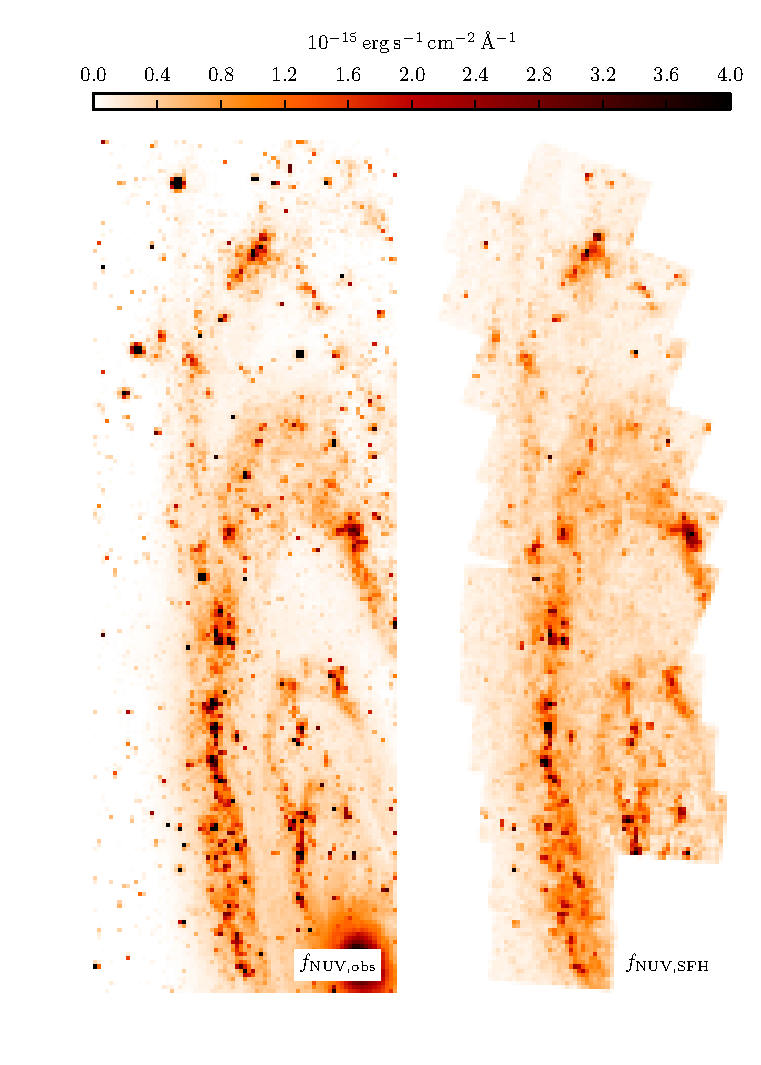
\includegraphics[width=\textwidth]{m31flux-figures/fluxmaps_nuv.pdf}
\caption[Observed and synthetic reddened \nuv{} flux maps.]{Same as Figure
    \ref{fig:mfx:fluxmaps_fuv}, but for \nuv{} flux.
}
\label{fig:mfx:fluxmaps_nuv}
\end{figure}


\textbf{*** TODO}

\begin{enumerate}
\item Uncertainties? For statistical/Poisson uncertainties, divide the \fuv{}
    and \nuv{} intensity (count) maps by the CCD gain to convert the units into
    photons, and take the square root. Flux is proportional to photon rate, so
    the flux uncertainties are just a constant times the raw Poisson
    uncertainties. The uncertainties won't be useful for the map
    visualizations, but they will be important for scatter plots comparing the
    synthetic and observed fluxes.
\end{enumerate}

\textbf{***}





\section{SFR estimates}\label{mfx:sfrestimates}

A common method for estimating the SFR of a target is to measure the integrated
flux in one or more filters and then calculate the SFR using one of the
flux-to-SFR calibrations available in the literature, e.g., (for UV flux) those
discussed in \citet{Kennicutt:1998}, \citet{Salim:2007}, \citet{Hao:2011},
\citet{Murphy:2011}, and \citet{Leroy:2012}; see also the review by
\citet{Kennicutt:2012}. We used this method to derive SFR maps for the PHAT
survey area, which we can later compare with similar maps derived from the
\citet{Lewis:2014} SFH data, effectively extending the work of
\citet{Simones:2014} to a much larger and more diverse sample.

To calculate flux-based SFRs, we converted the \ffuvobs{} and \fnuvobs{} maps
into AB magnitudes (Table \ref{tab:mfx:filters}), \fuvobs{} and \nuvobs{},
which we corrected for extinction by subtracting the modeled \afuv{} and
\anuv{} maps (\S \ref{mfx:syntheticfluxmaps:fluxmod}). The extinction-corrected
maps were converted back into (specific) fluxes ($\erg \ssec^{-1} \cm^{-2}
\ang^{-1}$), then into total fluxes ($\erg \ssec^{-1} \cm^{-2}$) by multiplying
by the effective filter wavelength \citep[$1538.6\ang$ for \fuv{}, $2315.7\ang$
for \nuv{};][]{Morrissey:2007}, and then into luminosities \lfuv{} and \lnuv{}
($\erg \ssec^{-1}$) assuming a distance modulus of 24.47
\citep{McConnachie:2005}. Finally, we applied the calibrations from
\citet{Kennicutt:1998} with updates by \citet{Hao:2011} and \citet{Murphy:2011}
\citep[see the review by][]{Kennicutt:2012} to obtain the \fuv{} and \nuv{}
flux-based SFR estimates, \sfrfuv{} and \sfrnuv{}, respectively:
\begin{equation}
\left(\frac{\sfrfuv}{\msun\yr^{-1}}\right) = 10^{-43.35}\,\left(\frac{\lfuv}{\erg\ssec^{-1}}\right) \\
\end{equation}
\begin{equation}
\left(\frac{\sfrnuv}{\msun\yr^{-1}}\right) = 10^{-43.17}\,\left(\frac{\lnuv}{\erg\ssec^{-1}}\right)
\end{equation}
These calibrations are based on stellar population synthesis using Starburst99
\citep{Leitherer:1999} and assuming a constant SFR over the last $100\myr$, the
\citet{Kroupa:2001} IMF, a mass range of 0.1 to $100\msun$, and solar
metallicity \citep{Hao:2011}.

The most robust flux calibrations are the those that rely on more than one part
of the electromagnetic spectrum. For example, the combination of GALEX \fuv{}
and Spitzer $24\,\mu\mathrm{m}$ fluxes into a single hybrid estimator that
simultaneously accounts for the direct starlight from newly-formed massive
stars and the absorbed starlight processed and reradiated by dust
\citep[e.g.,][]{Leroy:2012}. We have limited our study to observations by
GALEX, however, so we will only consider the simpler monochromatic \fuv{} and
\nuv{} calibrations above. The final \sfrfuv{} and \sfrnuv{} maps are shown in
Figure \ref{fig:mfx:sfrmaps1}.


\begin{figure}
\centering
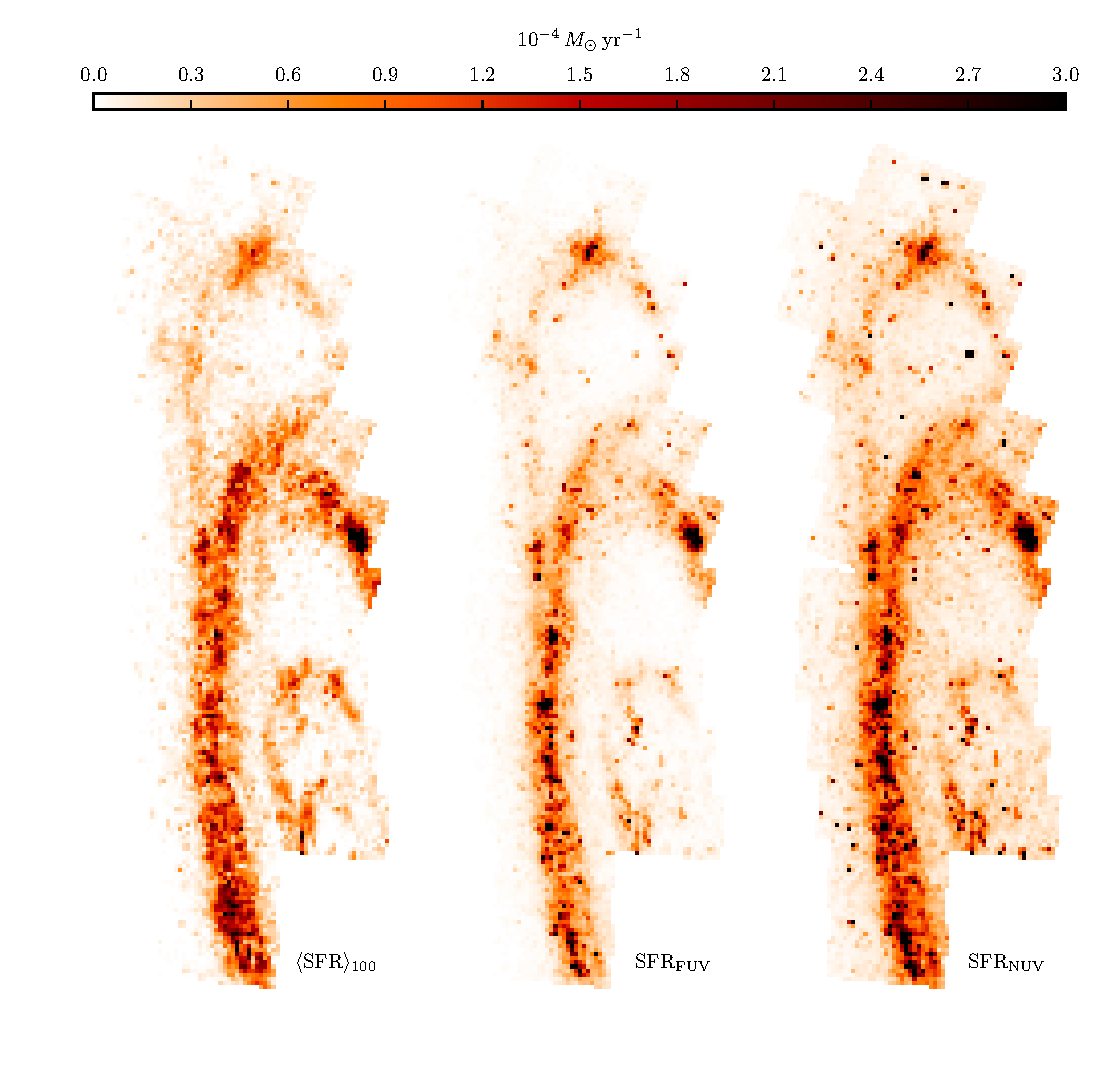
\includegraphics[width=\textwidth]{m31flux-figures/sfrmaps1.pdf}
\caption[SFR maps from estimates based on observed fluxes compared with the
    mean SFR map from the SFHs.]{\fuv{} and \nuv{} flux-based SFRs, \sfrfuv{}
    (middle) and \sfrnuv{} (right), compared with \sfroneh{} (left), the mean
    SFR over the last $100\myr$ of the SFHs. The flux-based SFRs were derived
    from the observed GALEX fluxes, \fuvobs{} and \nuvobs{} (Figures
    \ref{fig:mfx:fluxmaps_fuv} and \ref{fig:mfx:fluxmaps_nuv}), corrected for
    extinction using \afuv{} and \anuv{} (Figures \ref{fig:mfx:modfluxmaps_fuv}
    and \ref{fig:mfx:modfluxmaps_nuv}).
}
\label{fig:mfx:sfrmaps1}
\end{figure}


We also created a map for the mean SFR over the past $100\myr$ of the SFHs,
\sfroneh{}, which we show alongside the flux-based SFR maps in Figure
\ref{fig:mfx:sfrmaps1}. The $100\myr$ limit represents the nominal timescale of
UV emission and matches the timescale used by \citet{Hao:2011} to derive the
\fuv{} and \nuv{} flux calibrations.

Finally, we created another pair of \fuv{} and \nuv{} flux-based SFR maps
derived just as before, except we instead started the intrinsic synthetic flux
maps described in \S \ref{mfx:syntheticfluxmaps:fluxmod}. Because the fluxes
were intrinsic, we did not need to apply an extinction correction before
converting the fluxes into SFRs. The maps for the intrinsic flux-based SFR
estimates, \sfrfuvz{} and \sfrnuvz{}, are shown in Figure
\ref{fig:mfx:sfrmaps2}.


\begin{figure}
\centering
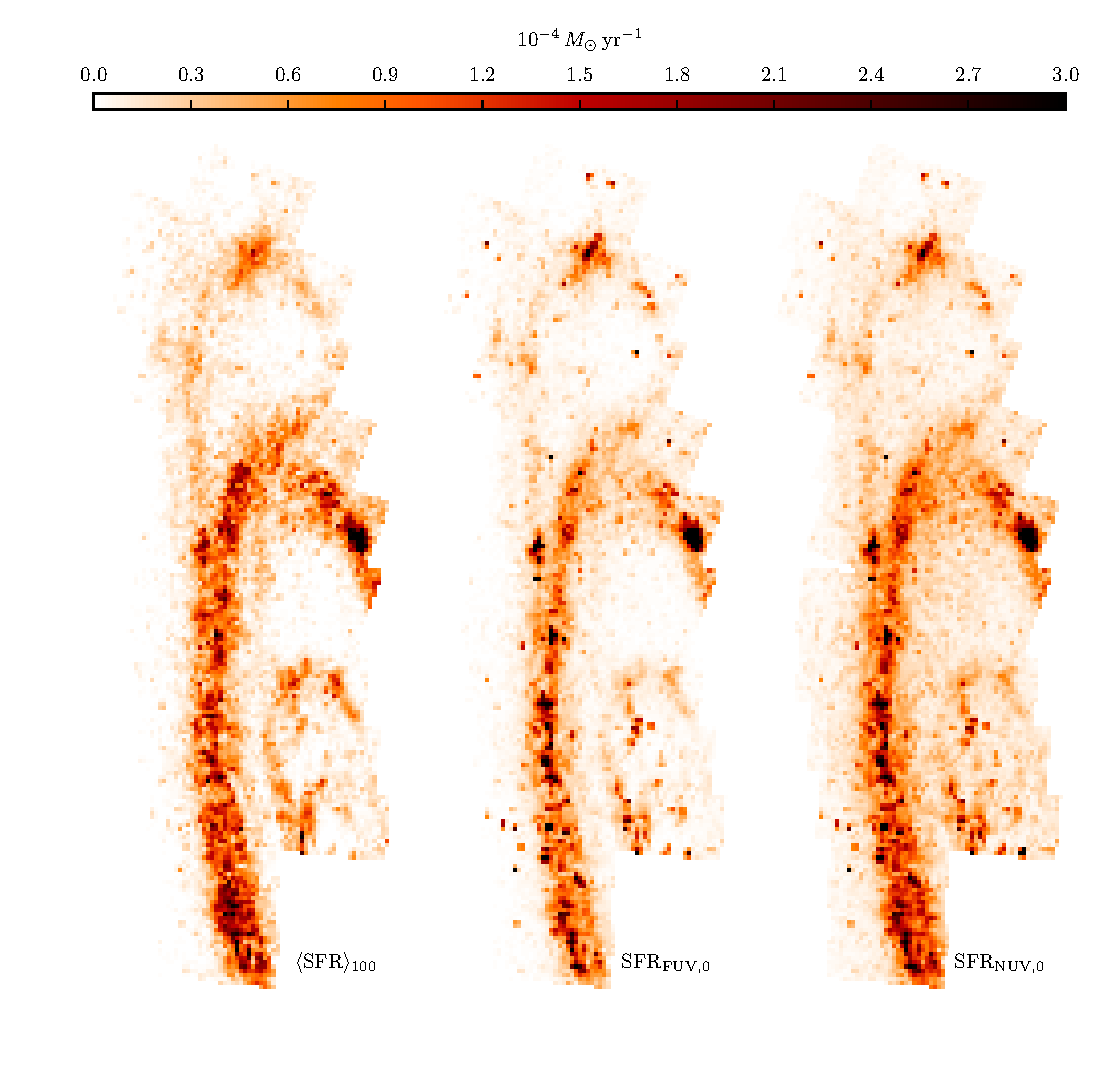
\includegraphics[width=\textwidth]{m31flux-figures/sfrmaps2.pdf}
\caption[SFR maps from estimates based on synthetic intrinsic fluxes compared
    with the mean SFR map from the SFHs.]{Same as Figure
    \ref{fig:mfx:sfrmaps1}, but instead comparing \sfroneh{} with \sfrfuvz{}
    and \sfrnuvz{}, the synthetic intrinsic (i.e., unreddened) fluxes from
    Figures \ref{fig:mfx:modfluxmaps_fuv} and \ref{fig:mfx:modfluxmaps_nuv}.
}
\label{fig:mfx:sfrmaps2}
\end{figure}





\section{Discussion}\label{mfx:discussion}

\subsection{Modeled flux}

\textbf{*** TODO}

\begin{enumerate}
\item Discuss the quality of the synthetic flux maps with respect to the
    observed flux maps.
\end{enumerate}

\textbf{***}


\begin{figure}
\centering
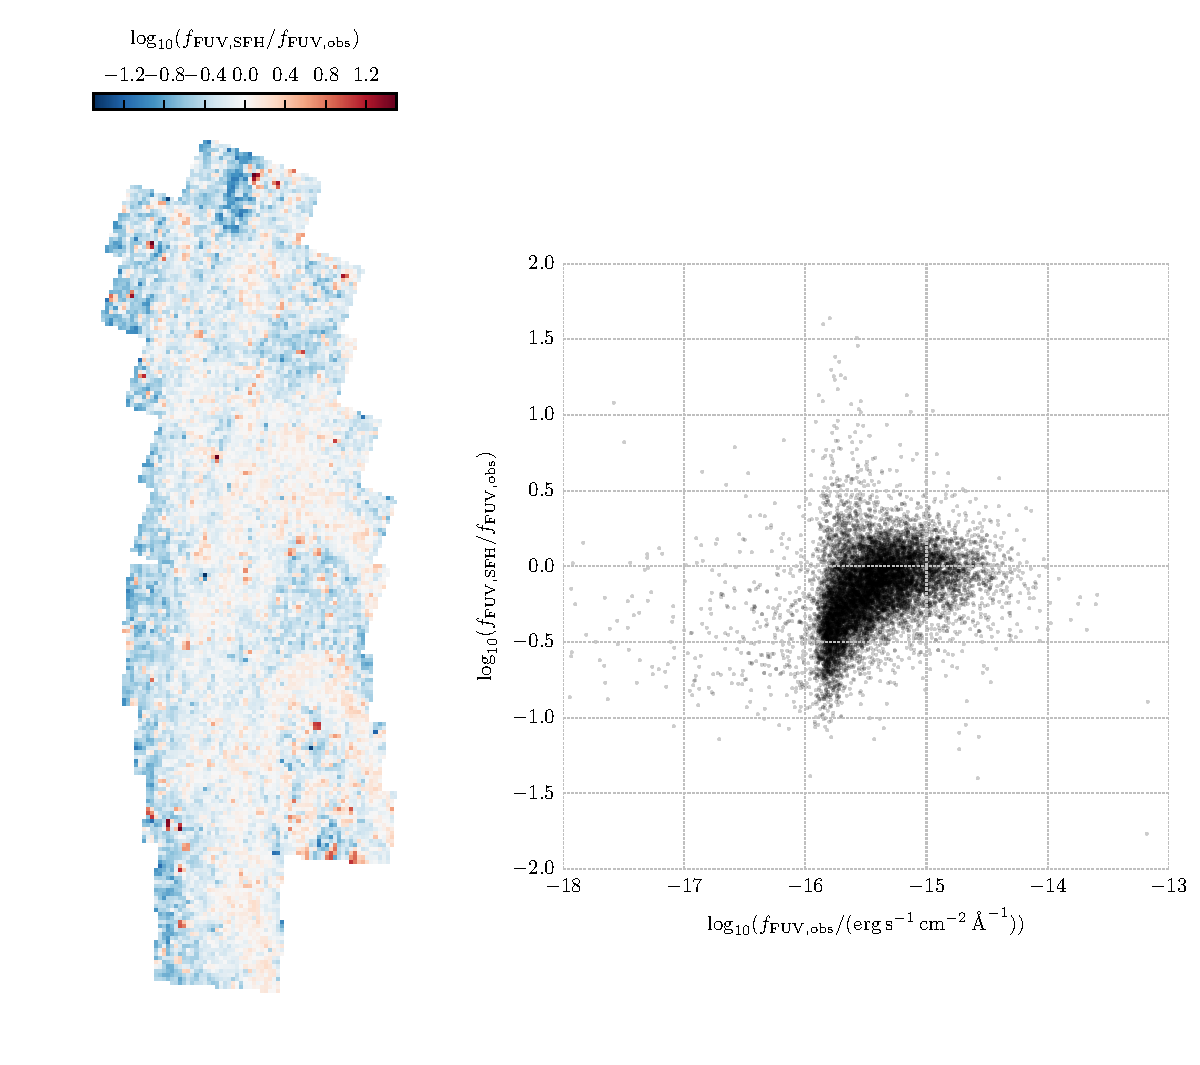
\includegraphics[width=\textwidth]{m31flux-figures/flux_fuv_sfh-vs-obs.pdf}
\caption[Ratio of the synthetic \fuv{} flux to the observed \fuv{} flux.]{Ratio
    of the synthetic \fuv{} flux to the observed \fuv{} flux.
}
\label{fig:mfx:fuvfluxratio}
\end{figure}


\begin{figure}
\centering
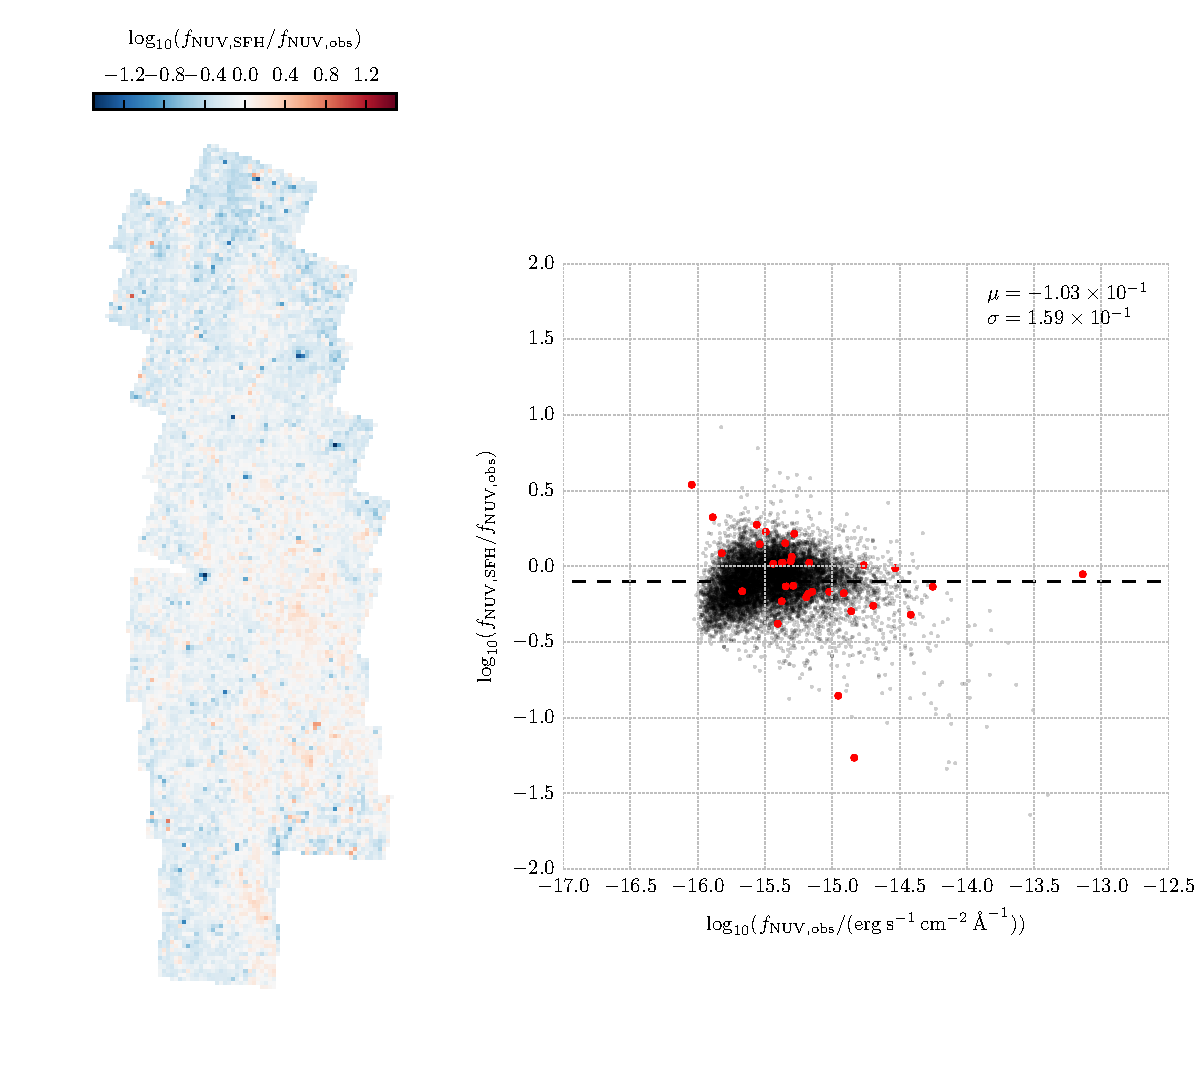
\includegraphics[width=\textwidth]{m31flux-figures/flux_nuv_sfh-vs-obs.pdf}
\caption[Ratio of the synthetic \nuv{} flux to the observed \nuv{} flux.]{Ratio
    of the synthetic \nuv{} flux to the observed \nuv{} flux.
}
\label{fig:mfx:nuvfluxratio}
\end{figure}



\subsection{SFR estimates from FUV flux}

\textbf{*** TODO}

\begin{enumerate}
\item Discuss the predicted flux-based SFRs with respect to the SFH-derived
    SFRs.
\end{enumerate}

\textbf{***}


\begin{figure}
\centering
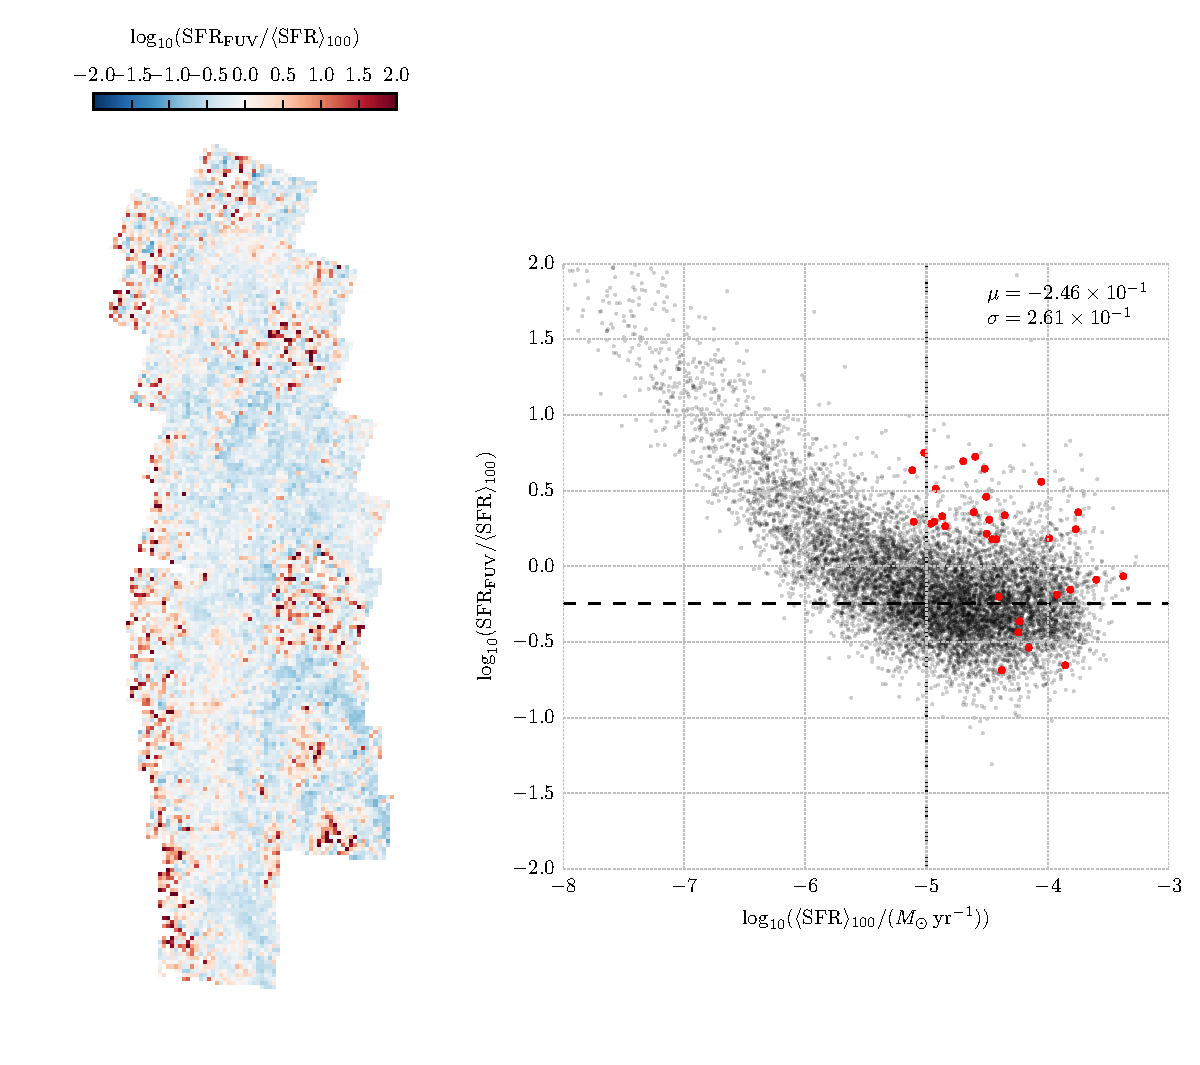
\includegraphics[width=\textwidth]{m31flux-figures/sfr_fuv-vs-mean.pdf}
\caption[Ratio of the \sfr{} based on the observed extinction-corrected \fuv{}
    flux to the $100\myr$ mean \sfr{}.]{Ratio of the \sfr{} based on the
    observed extinction-corrected \fuv{} flux to the $100\myr$ mean \sfr{}.
}
\label{fig:mfx:fuvsfrratio}
\end{figure}


\begin{figure}
\centering
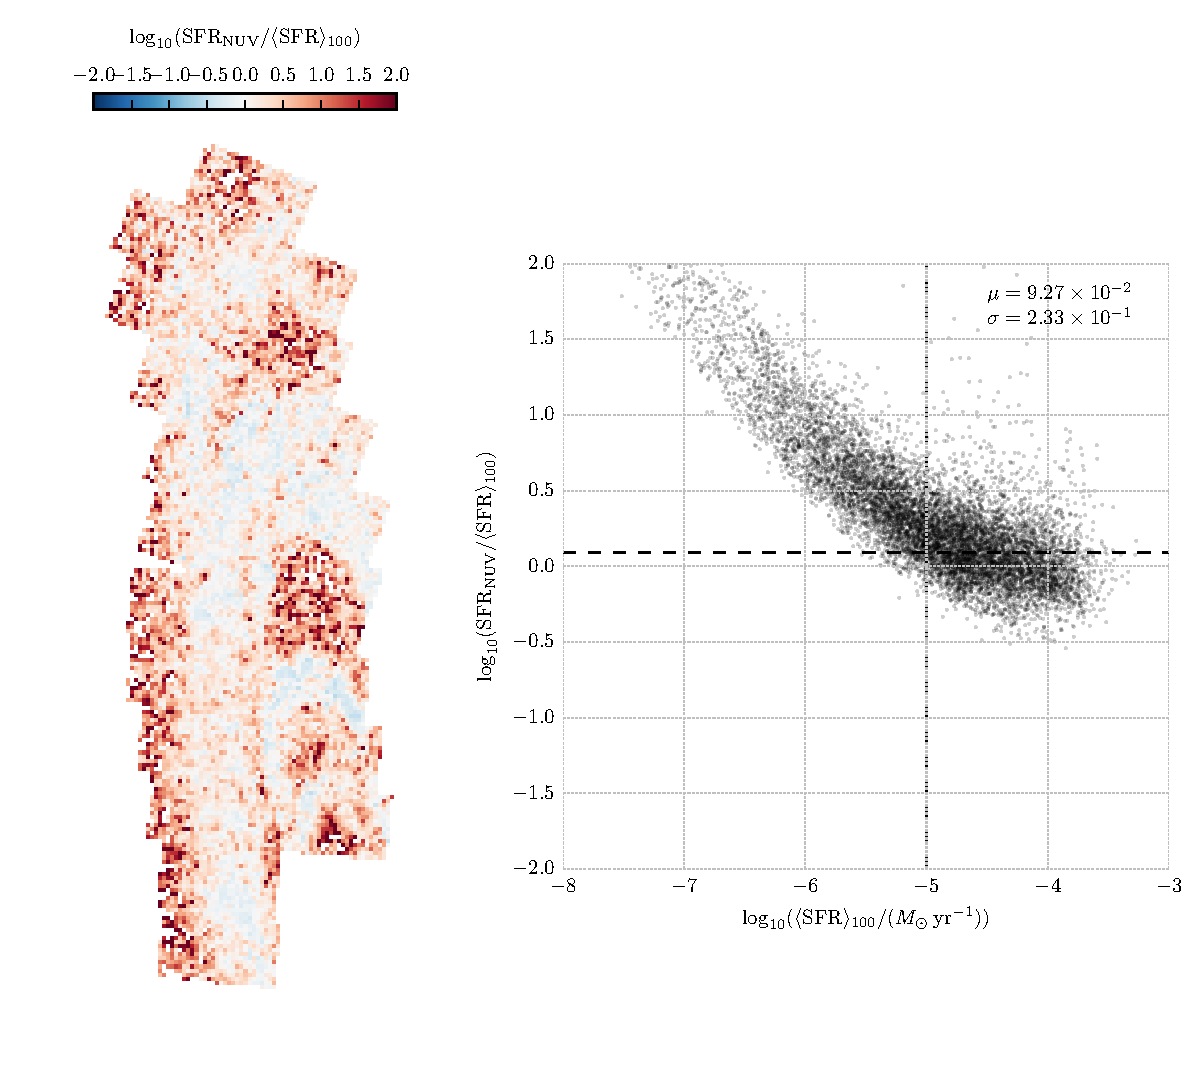
\includegraphics[width=\textwidth]{m31flux-figures/sfr_nuv-vs-mean.pdf}
\caption[Ratio of the \sfr{} based on the observed extinction-corrected \nuv{}
    flux to the $100\myr$ mean \sfr{}.]{Ratio of the \sfr{} based on the
    observed extinction-corrected \nuv{} flux to the $100\myr$ mean \sfr{}.
}
\label{fig:mfx:nuvsfrratio}
\end{figure}


\begin{figure}
\centering
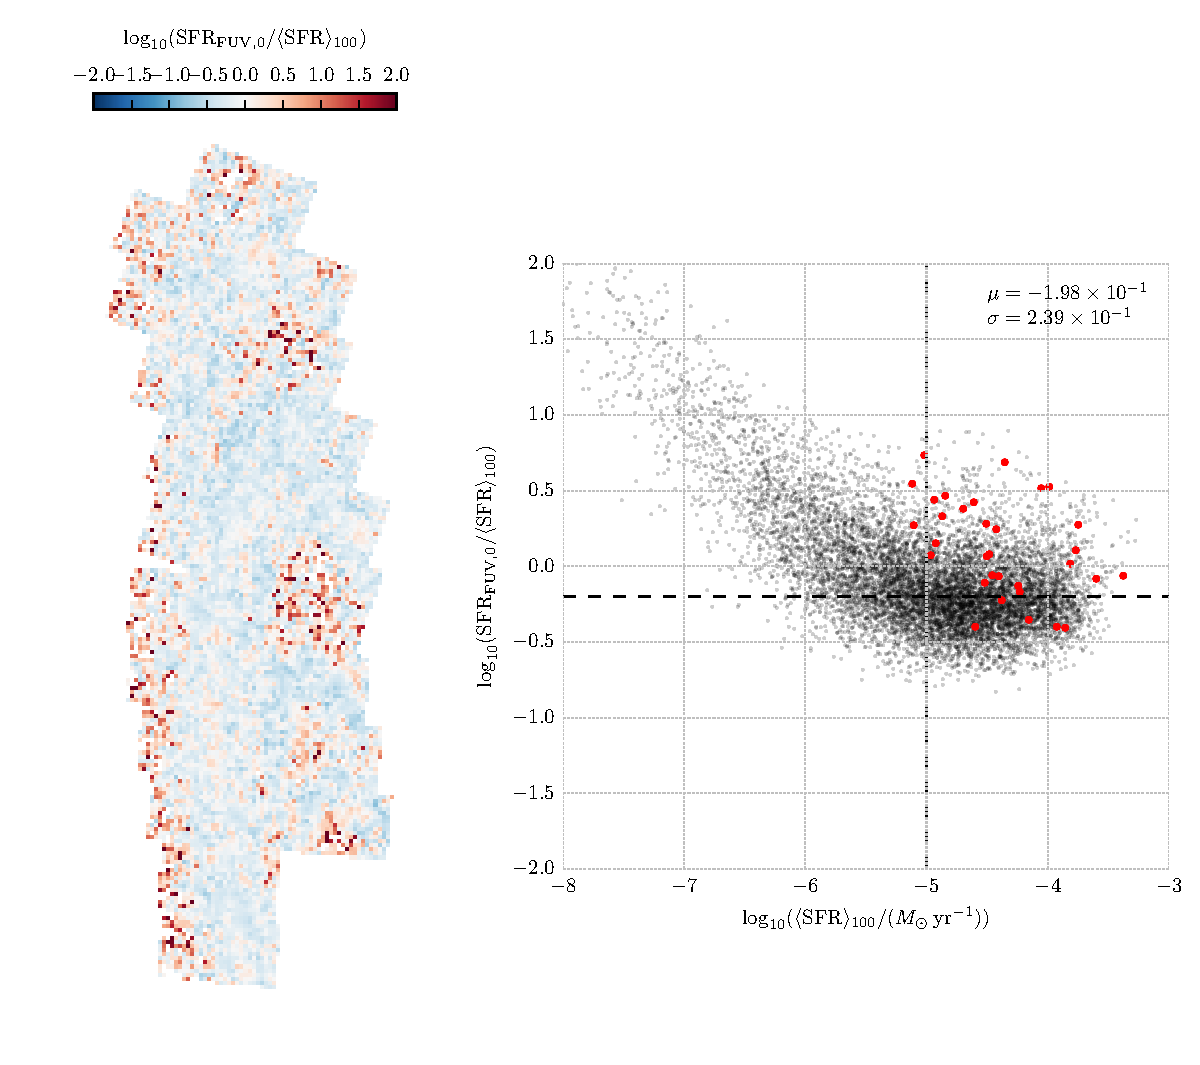
\includegraphics[width=\textwidth]{m31flux-figures/sfr_fuv0-vs-mean.pdf}
\caption[Ratio of the \sfr{} based on the synthetic intrinsic \fuv{} flux
    to the $100\myr$ mean \sfr{}.]{Ratio of the \sfr{} based on the synthetic
    intrinsic \fuv{} flux to the $100\myr$ mean \sfr{}.
}
\label{fig:mfx:fuvzsfrratio}
\end{figure}


\begin{figure}
\centering
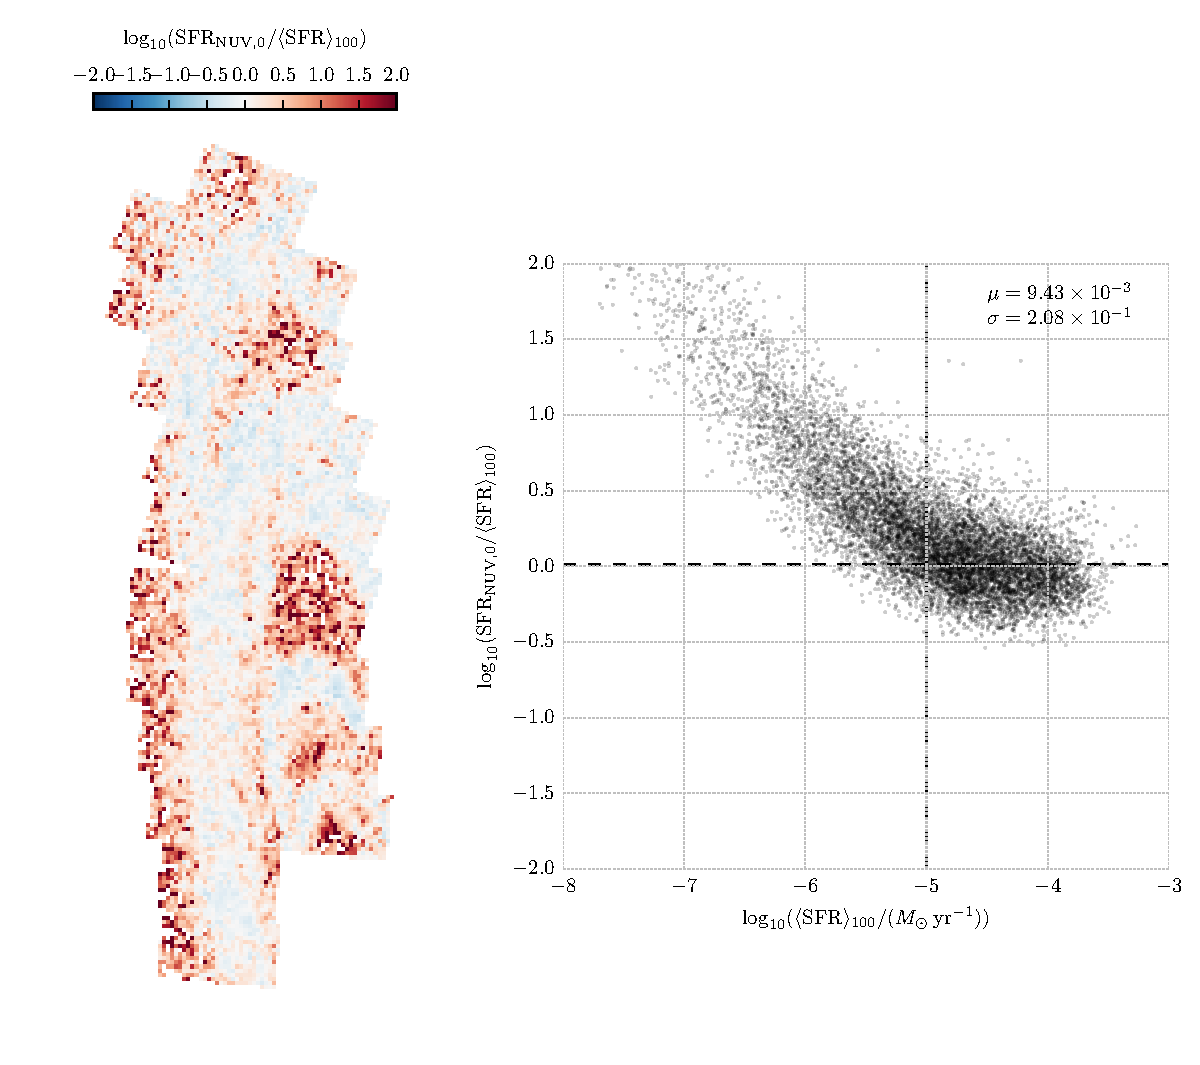
\includegraphics[width=\textwidth]{m31flux-figures/sfr_nuv0-vs-mean.pdf}
\caption[Ratio of the \sfr{} based on the synthetic intrinsic \nuv{} flux
    to the $100\myr$ mean \sfr{}.]{Ratio of the \sfr{} based on the synthetic
    intrinsic \fuv{} flux to the $100\myr$ mean \sfr{}.
}
\label{fig:mfx:nuvzsfrratio}
\end{figure}



\section{Conclusion}\label{mfx:conclusion}

Conclude.

This research made use of Montage, funded by the National Aeronautics and Space
Administration's Earth Science Technology Office, Computation Technologies
Project, under Cooperative Agreement Number NCC5-626 between NASA and the
California Institute of Technology. Montage is maintained by the NASA/IPAC
Infrared Science Archive.

\textbf{*** TODO}

\begin{enumerate}
\item Write this after the discussion and introduction are finished. Then
    write the abstract.
\end{enumerate}

\textbf{***}
